\begin{figure*}[t]
    \centering
    \vspace{3mm}
    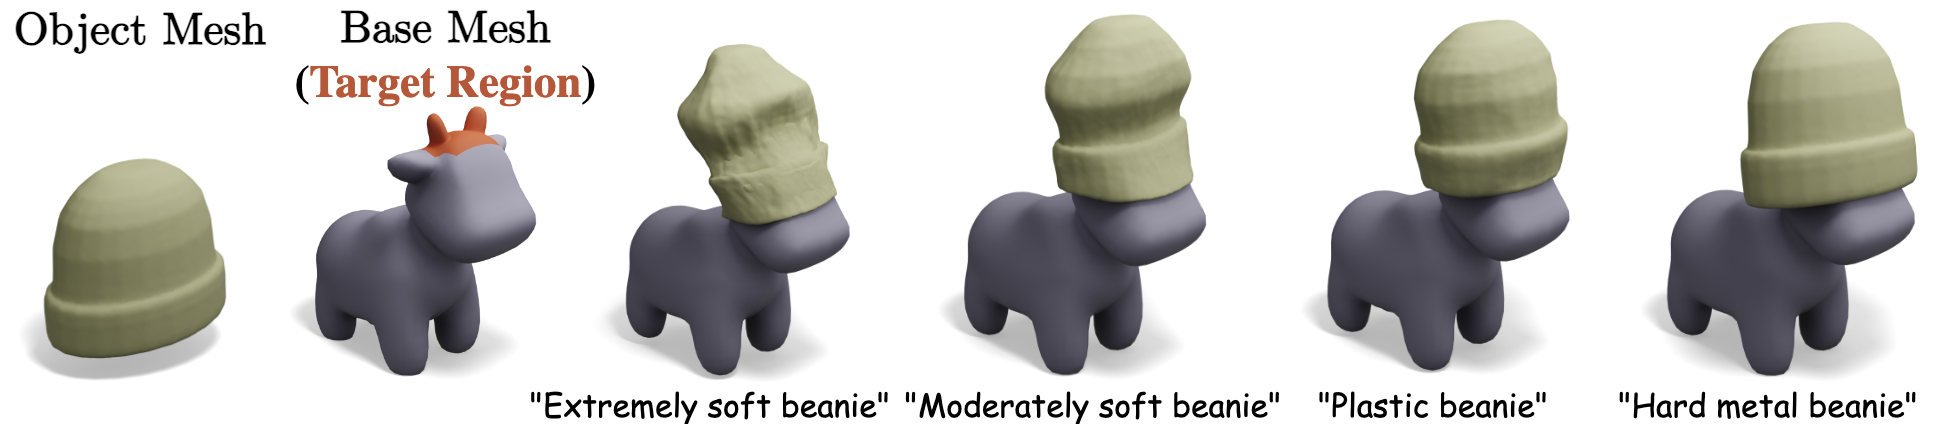
\includegraphics[width=\textwidth]{figures/materials/materials.png}
    \captionof{figure}{\ourmethod{} is capable of fitting the accessory onto the base mesh in a way that considers material properties. Instead of having to specify the numeric material parameters, artists can provide material guidance through text prompts, that get combined with rendered images and interpreted by a VLM to output specific elastic parameters.}
    %\vspace{-2cm}
    \label{fig:materials}
\end{figure*}%
